\renewcommand{\theequation}{\theenumi}
\begin{enumerate}[label=\arabic*.,ref=\thesubsection.\theenumi]
\numberwithin{equation}{enumi}

\item here
\begin{align}
\vec {P} - \vec {S} &=  \myvec{2\\2}
\\
\vec {Q} - \vec {P} &= \myvec{2\\2}
\end{align}
\begin{figure}[!ht]
	\centering
	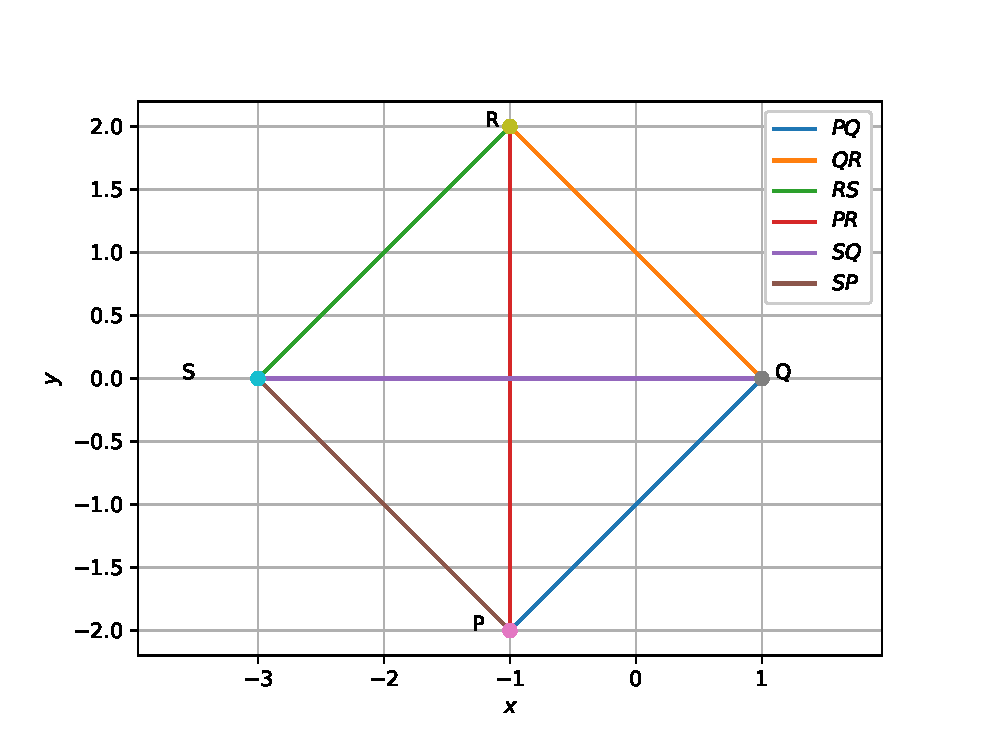
\includegraphics[width=\columnwidth]{./figures/line/quads/quad1.eps}
	\caption{quadrilateral1 }
	\label{fig:quadrilateral1}
	Path to the python code for the above figure
	\begin{lstlisting}
	codes/line/quad/quad1.py
	\end{lstlisting}
\end{figure}
\begin{align}
\vec{d1} &= \vec{R} - \vec{P} 
\\&= \myvec{0\\4}
\\
\vec{d2} &= \vec{S} - \vec{Q} 
\\&= \myvec{-4\\0}
\\
\norm{ \mathbf{\vec{d1}} \times \mathbf{\vec{d2}}} &= 
\norm{ \mathbf{\myvec{5\\1}} \times \mathbf{\myvec{1\\5}}} &= 16
\\
\norm{ \mathbf{\left(\vec {P} - \vec {S}\right)} \times \mathbf{\left(\vec {Q} - \vec {P}\right)}} &= \norm{ \mathbf{\myvec{2\\2}} \times \mathbf{\myvec{2\\2}}} &= 8
\\
\frac{1}{2}\norm{ \mathbf{\vec{d1}} \times \mathbf \vec{d2}} &= \norm{ \mathbf{\left(\vec {P} - \vec {S}\right)} \times \mathbf{\left(\vec {Q} - \vec {P}\right)}}&= 8
\end{align}
from above we can say that tha area of the quadrileteral is equal to the half of the multiplication of its diogonals.thus this is a rhombus.




\item 
\begin{align}
\vec{Q} - \vec{P} &= \myvec{6\\-4}
\\
\vec{R} - \vec{P} &= \myvec{3\\-2}
\\
\vec{Q} - \vec{R} &= \myvec{3\\-2}
\\
\left(\vec{Q} - \vec{P}\right) &= \left(\vec{R} - \vec{P}\right) + \left(\vec{Q} - \vec{R}\right) 
\\&= \myvec{6\\-4}
\end{align}
so from above we can say that $\vec P,\vec Q$ and $\vec R$ are linear so it can not be a quadrilateral.

\begin{figure}[!ht]
	\centering
	\includegraphics[width=\columnwidth]{./figures/line/quads/quad2.eps}
	\caption{quadrilateral2 }
	\label{fig:quadrilateral2}
	Path to the python code for the above figure
	\begin{lstlisting}
	codes/line/quad/quad2.py
	\end{lstlisting}
\end{figure}

\item
\begin{align}
\vec{Q} - \vec{P} &= \myvec{3\\1}
\\
\vec{R} - \vec{S} &= \myvec{3\\1}
\\
\vec{P} - \vec{S} &= \myvec{3\\3}
\\
\vec {Q} - \vec {R} &= \myvec{3\\3}
\\
\left(\vec{Q} - \vec{P}\right) &= \left(\vec{R} - \vec{S}\right)
\\
\left(\vec{P} - \vec{S}\right) &= \left(\vec{Q} - \vec{R}\right)
\end{align}
Thus above equations shows that the opposites sides are parallel and equal in length
\begin{align}
\vec{d1} &= \vec{R} - \vec{P} 
\\&= \myvec{0\\-2}
\\
\vec{d2} &= \vec{S} - \vec{Q} 
\\&= \myvec{-6\\-4}
\\\norm{ \mathbf{\vec{d1}} \times \mathbf{\vec{d2}}} &= 
\norm{ \mathbf{\myvec{5\\1}} \times \mathbf{\myvec{1\\5}}} 
\\&= 8
\\
\norm{ \mathbf{\left(\vec {P} - \vec {S}\right)} \times \mathbf{\left(\vec {Q} - \vec {P}\right)}} &= \norm{ \mathbf{\myvec{2\\2}} \times \mathbf{\myvec{2\\2}}}
\\ &= 10
\\
\norm{ \mathbf{\left(\vec {P} - \vec {S}\right)} \times \mathbf{\left(\vec {Q} - \vec {P}\right)}} &\neq \norm{ \mathbf{\left(\vec {P} - \vec {S}\right)} \times \mathbf{\left(\vec {Q} - \vec {P}\right)}}
\end{align}
From equation (3.1.3.5),(3.1.3.6)and (3.1.3.15) we can say that 
it is a parallelogram.
\end{enumerate}
\begin{figure}[!ht]
	\centering
	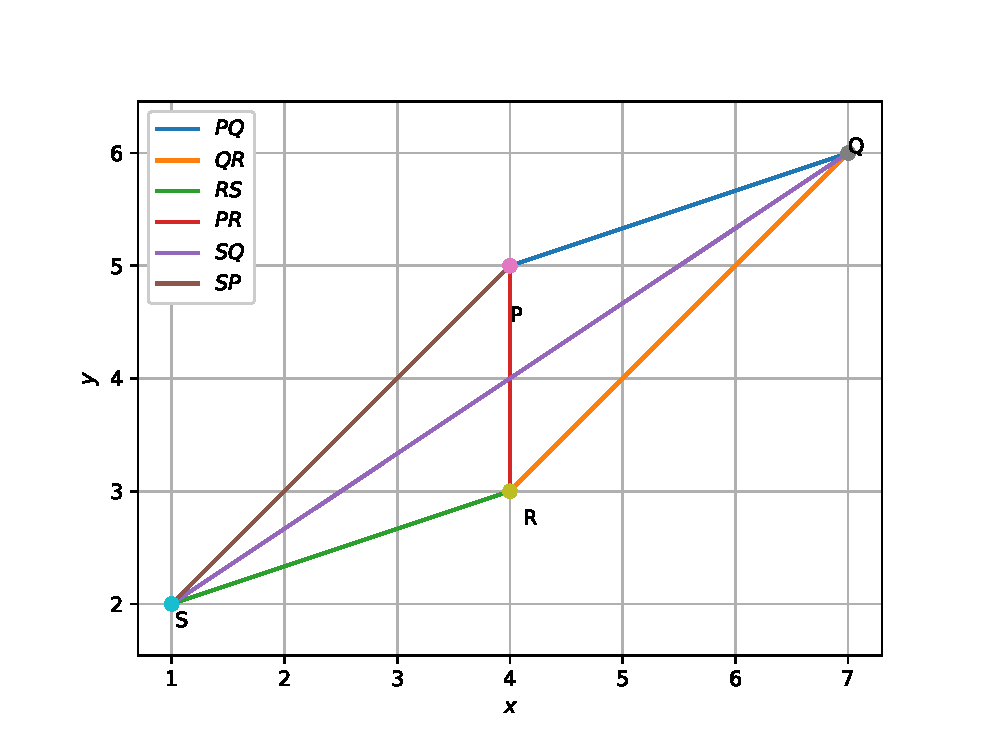
\includegraphics[width=\columnwidth]{./figures/line/quads/quad3.eps}
	\caption{quadrilateral3 }
	\label{fig:quadrilateral2}
	Path to the python code for the above figure
	\begin{lstlisting}
	codes/line/quad/quad3.py
	\end{lstlisting}
\end{figure}

